\documentclass[11pt]{article}


%\documentclass[11 pt]{article}
\usepackage{graphicx}
\usepackage{float}



\usepackage[utf8]{inputenc}

\usepackage[square,sort,comma,numbers]{natbib}
\bibliographystyle{abbrvnat}
\setcitestyle{authoryear,open={(},close={)}} %Citation-related commands

\usepackage{setspace}

\usepackage{pdflscape}
%\doublespacing
\onehalfspacing
\usepackage[dvipsnames]{xcolor}
\usepackage{lineno}
\linenumbers
\usepackage{multicol}
\usepackage{hyperref}
\hypersetup{
	colorlinks=false,
%	linkcolor=blue,
%	filecolor=magenta,      
%	urlcolor=cyan,
	pdftitle={Overleaf Example},
	pdfpagemode=FullScreen,
}

\addtolength{\oddsidemargin}{-2.5cm}
\addtolength{\evensidemargin}{-1.5cm}

\addtolength{\textwidth}{5.5cm}

\addtolength{\topmargin}{-.875in}
\addtolength{\textheight}{1.75in}

%\author{Pending}


\begin{document}
%\title{Understanding the emergence of viral variants of concern via Bayesian molecular clock model selection}
\begin{flushright}

%\today
\end{flushright}
\begin{center}
	\begin{LARGE}
	\textbf{The phylodynamic threshold of measurably evolving populations}
	\end{LARGE}

Ariane Weber$^{1,*}$, Sanni Översti$^{1}$, Julia Kende$^{2}$, and Sebastian Duchene$^{3,4,*}$.
\end{center}

$^{1}$ Pending.

$^{2}$ Institut Pasteur, Université Paris Cité, Bioinformatics and Biostatistics Hub, Paris, France.

$^{3}$ ED-ID unit, Dept of Computational Biology, Institut Pasteur, Paris, France.

$^{4}$ Peter Doherty Institute for Infection and Immunity, Dept of Microbiology and Immunology, University of Melbourne, Melbourne, Australia.


*email: weber@gea.mpg.de, sduchene@pasteur.fr
%		\maketitle
\newline

\begin{Large}
	\textbf{Abstract}
\end{Large}

Pending.

\textbf{Keywords:} Measurably evolving populations, phylodynamic threshold, molecular clock, Bayesian phylogenetics, microbial evolution.

%\begin{Large}
%\textbf{Significance statement}
%\end{Large}

%Genome data from the ongoing SARS-CoV-2 pandemic have been key to detect and trace the emergence of variants of concern, with increase transmissibility and impacts on vaccine efficacy. At a genetic level, variants have much higher numbers of defining mutations than is expected under the standard mutation rate of the virus. We analysed genome data of the four variants of concern recognised by the WHO to uncover their evolutionary dynamics. We find that the lineages of the virus that preceded these variants had a mutation rate at least 4 times faster than the baseline, a process that was sustained over a few months, but which does not appear permanent.
%Up to 120 words. 

\section{Introduction}
Molecular sequence data have become nearly ubiquitous for studying the evolution of modern and ancient organisms. A fundamental concept in molecular evolution is the `molecular clock', which posits that substitutions accumulate roughly constantly over time \citep{zuckerkandl1965evolutionary}. An underlying assumption of the classic molecular clock is that selective constraints are negligible for most sites and over time. The development of molecular clock models as statistical processes relaxes this and other assumptions by allowing for rate variation among branches in phylogenetic trees (reviewed by \cite{ho2014molecular}).

Molecular clock models necessarily involve two key quantities, the evolutionary timescale and the `evolutionary rate', with the latter representing the combination of mutations and substitutions that accrue over time. However, evolutionary times and rates are undeniable (\cite{dos2013unbearable}, as reviewed by \cite{bromham2018bayesian}), and therefore cannot be jointly identified using genetic sequence data alone. To make inferences about them from genetic sequences, all molecular clock methods require prior assumption about evolutionary times or rates, known as a `molecular clock calibration'. For example, one can constrain the age of the common ancestor between two lineages (i.e. an internal node in a phylogenetic tree) to a given time or fix the evolutionary rate to a known value. The choice of calibration depends on the information available and its reliability \citep{warnock2012exploring, duchene2014impact}. 

\subsection{Measurably evolving populations}
Rapidly evolving organisms, notably viruses and some bacteria, have been found to accrue an appreciable number of mutations over the sampling timescale. Influenza viruses, for example, have evolutionary rates of around $6\times10^{-3}$ subs/site/year \citep{ghafari2021purifying, sanjuan2012molecular}. Assuming a genome size of 13,500 Kb, one would expect to observe one mutation every 4 to 5 days ($\frac{365\ days/year}{13,500\ sites\ \times\ 6\times10^{-3}subs/site/year}\approx4.5\ days/subs$). If genome samples are collected over the course of a few weeks, then the sampling times themselves can be used to calibrate the molecular clock, a practice known as `tip calibration' (reviewed by \cite{rieux2016inferences}). Data sets for which the molecular clock can be calibrated using sequence sampling times are considered to have been sampled from a `measurably evolving population' \citep{drummond2003measurably}.

Advances in sequencing technologies have dramatically expanded the range of organisms from which data sets can be considered to have been sampled from a measurably evolving population. First, ancient DNA techniques have effectively expanded the genome sampling window for many organisms \citep{spyrou2019ancient, duchene2020recovery}. One of many examples, is mitochrondrial DNA recovered from dogs from 36,000 years before present \citep{thalmann2013complete}, which was found to be sufficient to calibrate its molecular clock. Second, whole genome sequencing has meant that data sets of `slowly' evolving microbes often carry sufficient information for calibrating the molecular clock \citep{biek2015measurably}. The causative agent of tuberculosis, the bacterium \textit{Mycobacterium tuberculosis}, was commonly considered to evolve too slowly for calibrating the molecular clock using samples collected over a few years \cite{duchene2016genome}. However, data sets involving the full genome, of about 4.4 Mb, have demonstrated that a genome sampling window of a few decades might be sufficient for reliable clock calibration \citep{menardo2019molecular}.

\subsection{The phylodynamic threshold}
The emergence of SARS-CoV-2 saw the rapid generation of genome data from the early stages of the outbreak, with phylodynamic analyses conducted in near to real-time \citep{attwood2022phylogenetic}. The first attempts to estimate the evolutionary rate and time of origin were highly uncertain due to two factors; a narrow sampling window and low genetic diversity. In \cite{duchene2020temporal} Bayesian phylodynamic analyses of the available genomes were conducted as the outbreak unfolded, such that the number of genomes and the width of the sampling window increased over time and ranged from 22 genomes sampled over 31 days to 122 genomes sampled over 63 days.  Early estimates of the evolutionary rate and time of origin had high uncertainty, but they rapidly converged to values that were robust to the addition of more data. The term `phylodynamic threshold' refers to the time where an organism has accrued a sufficient amount of genetic change \textit{since its emergence} for tip-calibrations to be informative \citep{duchene2020temporal}.

The minimum requirement for tip-calibrations to be informative is that there should be at least one mutation over the sampling period. For a given organism, the minimum sampling period can be calculated as the inverse of the product of genome size and the evolutionary rate (i.e. $\frac{1}{genome\ size\ (sites) \times evol.\ rate (subs/site/year)}=$ years to observe one mutation). We refer to this amount of time as the minimum expected phylodynamic threshold.

The terms \textit{phylodynamic threshold} and \textit{measurably evolving population} are different, albeit related, concepts. A population is measurably evolving if the samples available are sufficiently informative as to warrant tip calibration. In contrast, the phylodynamic threshold is the amount of time over which we would need to draw samples after the emergence for them to behave as from a measurably evolving population. For a recently evolving pathogen the phylodynamic threshold would simply correspond to the time until it can be considered a measurably evolving population, under the condition that the data have been collected constantly over time. In contrast, an ancient organism may have reached its phylodynamic threshold, with substantial genetic diversity since its emergence, but drawing samples from a very short time window may fail to capture a representative amount of such genetic diversity (Fig. \ref{figure:Fig1}).

\subsection{Temporal signal}
Tests of temporal signal are designed to assess our ability to extract information from data for estimating evolutionary rates and timescales (reviewed by \cite{rieux2016inferences}). These tests do not differentiate between recently emerging organisms (i.e. they have not attained their phylodynamic threshold; fig. \ref{figure:Fig1}a) and those with narrow sampling windows (i.e. the data cannot be treated as being drawn from a measurably evolving population; fig. \ref{figure:Fig1}d), both of which may lack temporal signal. Additionally, these tests assume that the phylogenetic model adequately captures the evolutionary process. However, pervasive evolutionary rate variation (an 'overdispersed molecular clock') may lead to rejection of temporal signal under a strict clock model. Thus, temporal signal is not solely a property of the data but also depends on model performance. Recent research suggests that the choice of tree prior and molecular clock model significantly impacts the sensitivity and specificity of temporal signal tests, with relaxed molecular clocks being particularly effective \citep{tay2024assessing}.

Various methods exist for assessing temporal signal, including root-to-tip regression \citep{buonagurio1986evolution, gojobori1990molecular, drummond2003inference}, date-randomization tests \citep{ramsden2009hantavirus, duchene2015performance, duchene2018inferring, trovao2015host}, and the Bayesian Evaluation of Temporal Signal (BETS; \cite{duchene2020bayesian}). Root-to-tip regression fits a regression to the distance from the root to the tips in a phylogenetic tree against sampling time sampling time, with the $R^2$ value indicating clocklike behavior. Date-randomization tests compare evolutionary rate estimates using correct sampling times against permutations. BETS evaluates whether a model with sampling times performs better than a model that assumes isochronous sampling using Bayes factors. Importantly, a lack of temporal signal does not necessarily preclude estimating evolutionary rates and timescales, as additional sources of information (e.g., prior rate estimates or known internal node ages) can provide valid calibration, although potentially less precise than sequence sampling times for microbial pathogens.

A lack of temporal signal is typically considered to be associated with unreliable molecular clock estimates. In practice, this situation is believed to be alleviated by broadening the sampling window or including more ancient samples. However, the presence and direction of a possible bias in estimates of evolutionary rates and timescales is poorly understood. 


%Tests of temporal signal were devised to determine our ability to draw information from the data to estimate evolutionary rates and timescales. Fundamentally, these tests do not make the distinction between organisms that are recently emerging (i.e. they have not attained their phylodynamic threshold; fig \ref{figure:Fig1}a) or those for which the sampling window is too narrow (i.e. the data cannot be treated as being drawn from a measurably evolving population; Fig \ref{figure:Fig1}d). 

%Moreover, tests of temporal signal make the assumption that evolutionary process is reasonably well captured by the phylogenetic model. If evolutionary rate variation is pervasive, known as an `overdispersed molecular clock' then a testing for temporal signal under a strict molecular clock model may reject temporal signal. Thus, temporal signal is not an inherent property of the data, but a combination of the information in the data and the performance of the model. In fact, recent research has suggested that the choice of the tree prior and molecular clock model can considerably impact the sensitivity and specificity of tests of temporal signal, with the relaxed molecular clock being particularly effective \citep{tay2024assessing}.

%The simplest method to assess temporal signal is the root-to-tip regression \citep{buonagurio1986evolution, gojobori1990molecular, drummond2003inference}, which consists of fitting a regression of the distance from the root to the tips as a function of the sampling time. The coefficient of determination, $R^2$, measures the degree of clocklike behaviour, and the regression parameters, slope and x-intercept correspond to estimates of the evolutionary rate and age of the root node, respectively. This method is very popular, with a range of user-friendly implementations \citep{rambaut2016exploring, featherstone2024clockor2}. However, the data points in the root to tip regression are not statistically independent, and therefore p-values are generally not reported. For this reason this method is used as a visual inspection, rather than a formal statistical test of temporal signal.

%Other tests of temporal signal test the association between sampling times and genetic divergence. The date-randomisation test \citep{ramsden2009hantavirus} consists of comparing the estimate of the evolutionary rate with the correct sampling times and with multiple permutations of the sampling times. The analysis of the data is considered to have temporal signal if the estimate with the correct sampling times does not overlap with the permutations. This test is available in Bayesian and maximum likelihood frameworks, and thus it benefits from a a range of molecular clock models \citep{duchene2015performance, duchene2018inferring, trovao2015host}.

%The Bayesian Evaluation of Temporal Signal, BETS, is an approach that is grounded on formal model testing \citep{duchene2020bayesian}. The premise of this test is whether the inclusion of sampling times in a Bayesian phylogenetic model improves results in better performance than their exclusion, where model performance is typically quantified using Bayes factors. Like the date-randomisation tests, BETS can exploit the full range of Bayesian phylogenetic models.

%Critically, a lack of temporal signal under any of the approaches above means that sampling times are not informative under the model in question, but this situation does not necessarily preclude a researcher from fitting a molecular clock and estimating evolutionary rates and timescales. Additional sources of information, such as prior evolutionary rate estimates for closely related organisms or known ages of internal nodes (and fossils where available) are entirely valid sources of calibration \citep{zhang2016total}, although they might be less precise than sequence sampling times, especially for microbial pathogens.

\begin{landscape}
	\begin{figure}[H]
		\begin{center}
			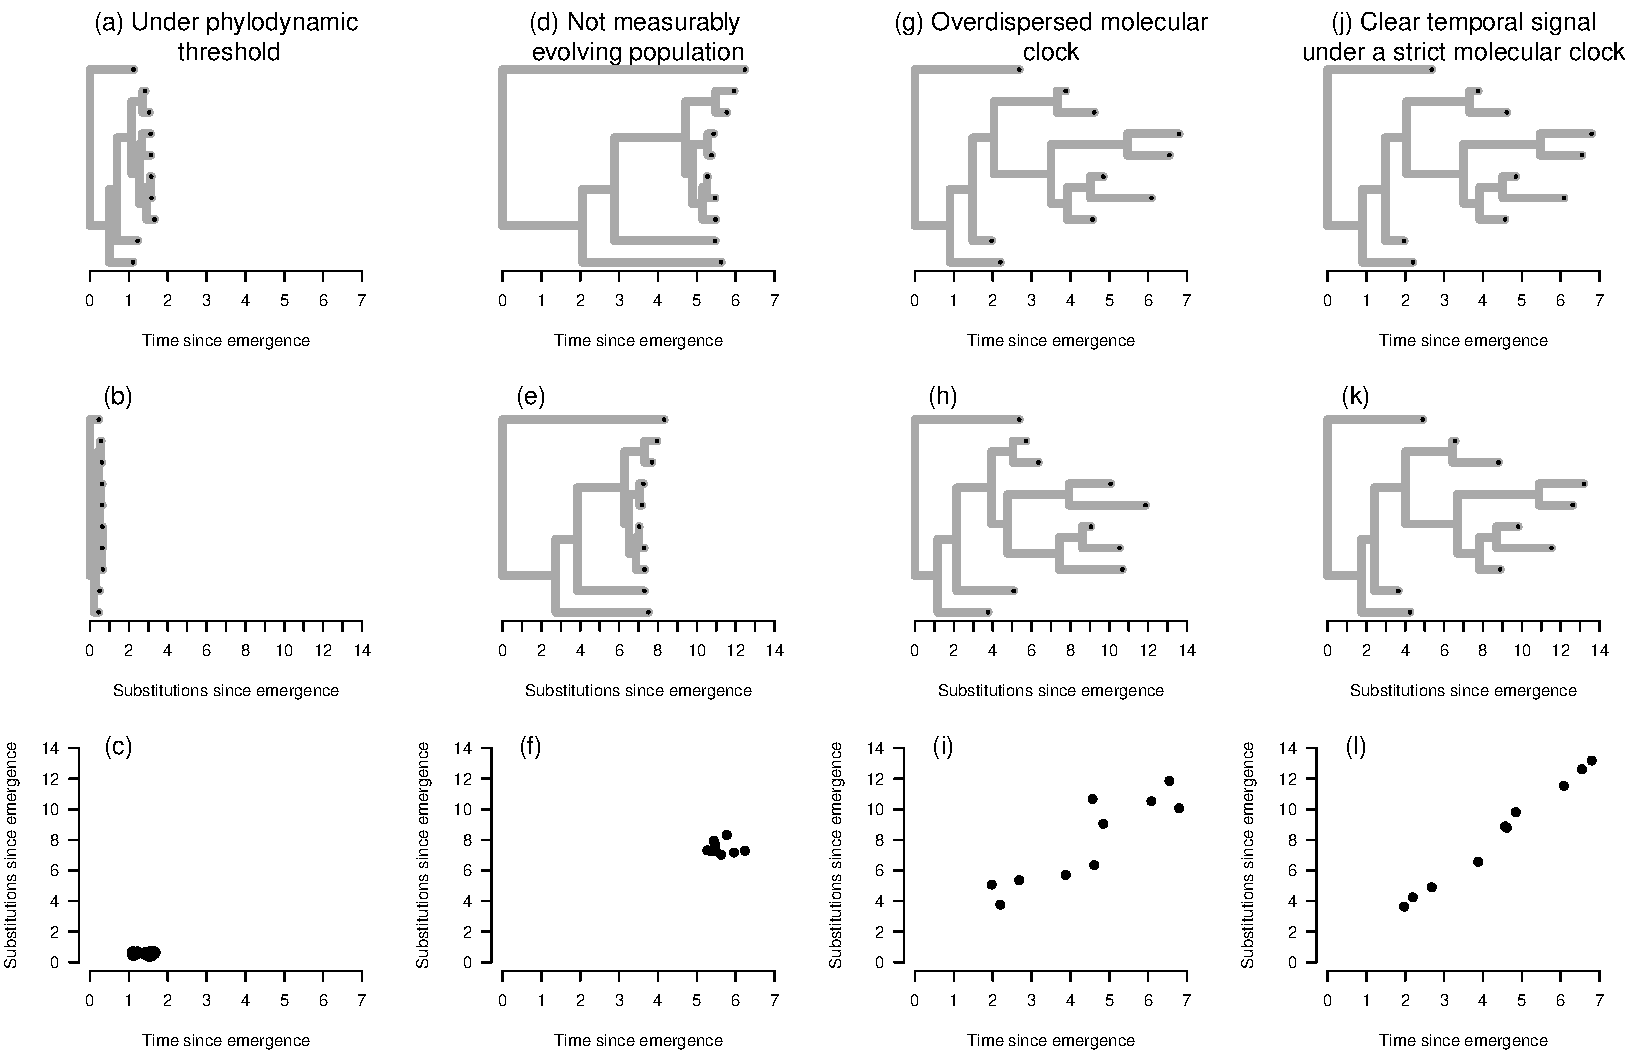
\includegraphics[scale=0.7, angle=0]{examples_temp_signal_thresholds_meps.pdf}
			\caption{Examples of situations where temporal signal is typically not detected. An organism that has not attained its phylodynamic threshold has a recent time of emergence (with a phylogenetic time tree shown in (a)) because it has not had sufficient time to accrue an appreciable number of substitutions (phylogenetic tree with branch lengths in subs/site, i.e. a `phylogram', shown in (b)), such that it is not possible to establish a statistical relationship between molecular evolution (substitutions) and time (shown in (c)). Sequence data from an organism that has evolved for a substantial amount of time may have been sampled over a very narrow window of time that is not sufficient to treat it as a measurably evolving population (time tree in (d) and phylogram in (e)), which results in no temporal signal (root-to-tip regression in (f)). A data set may involve a wide sampling window of time and from a population that has attained its phylodynamic threshold, but an overdispersed molecular clock (substantial rate variation among lineages; panels (g) - (i)) may result in a lack of temporal signal. In (j) through (l) we show the situation where an organism has attained its phylodynamic threshold and it has been sampled for sufficiently long, as to produce a clear relationship between molecular evolution and time, and unequivocal temporal signal.}
			\label{figure:Fig1}
		\end{center}
		%		\centering
	\end{figure}
\end{landscape}


\section{Results}
In this study we sought to pinpoint the impact of sampling strategies on these estimates. We focused our attention on two major problems for emerging microbes and studies involving ancient DNA. First, we varied the sampling window of a population that has attained its phylodynamic threshold. Second, we subsampled a population over time to vary the number of ancient samples, leading to a temporal sampling bias. Finally, we illustrate these results in an empirical data set of Hepatitis B virus (HBV) that includes a large number of ancient samples \citep{kocher2021ten}. This virus has been the subject of intense research due to its close association with human populations and complex evolutionary dynamics \citep{paraskevis2013dating, ross2018paradox, kahila2012tracing}.

\subsection{Sampling windows relative to the phylodynamic threshold}
We simulated sequence data that resembled the evolution of HBV, a double-stranded DNA (dsDNA) virus that has evolved in humans for around 10 thousand years \citep{kocher2021ten}. Our synthetic data had a genome length of 3,200 nucleotides and an evolutionary rate of $1.5\time10^{-5}$ subs/site/year \citep{kocher2021ten, muhlemann2018ancient}. Under these conditions we expect to observe one mutation every 20 years ($\frac{1}{3,200\ sites \times\ 1.5\times10^{-5}subs/site/year}\approx20\ years$). This number is important for the design of our simulation experiments: 20 years is the time we would expect for it to attain its phylodynamic threshold and it would typically be the required sampling window to detect temporal signal. We analysed the data under a Bayesian phylogenetic framework an considered whether the posterior contained the true value used to generate the data, known as coverage, and the width of the posterior, known as precision (a `precise' estimate has a narrow posterior distribution).

\subsection{Calibration windows for tips}
We conceived a simulation process under which the evolutionary timescale had an expected time of 10 thousand years and with a sampling window of 0, 10, 20, 200 , or 2,000 years. A sampling window spanning 0 years results in ultrametric trees with the sampling times providing no calibration information. In contrast, a sampling window of 10 years is half of the phylodynamic threshold and is expected to have weak temporal signal (see fig. \ref{figure:Fig1}(d)-(f)). Sampling windows of 20 years (the phylodynamic threshold) or wider are expected to behave as measurably evolving populations and with increasingly strong temporal signal (see fig. \ref{figure:Fig1}(j)-(l)). All our simulations were analysed under Bayesian phylogenetic framework, as implemented in the BEAST 2 platform \citep{bouckaert2019beast}.

All our simulations produced posterior estimated that included the correct value used to generate the data (i.e. 100\% coverage; fig. \ref{figure:Fig2}). Increasingly wide sampling windows improved the precision of the estimates, while still including the correct value. This result is unsurprising, given our configuration of the prior. Notably, the prior on the phylogenetic tree and the evolutionary rate are particularly influential for estimating evolutionary rates and timescales (for a detailed investigation see \cite{tay2024assessing}). Here, the tree prior is a constant-size coalescent for which the prior on the population size (known as $\Theta$) is an exponential distribution with mean of 5,000, which matches the value used to generate the data. Similarly, the evolutionary rate had a prior in the form of a $\Gamma$ distribution with $shape=1.5$ and $rate=10^{5}$, whose mean is $shape\times rate=1.5\times10^{-5}$ and thus also matches the `true' value. Although these priors are centred on the correct values, they are vague, and it is important to note than in all cases, the posterior distribution of the evolutionary rate and tree height was narrower than the prior, meaning that even in the absence of sampling times the sequence data provide some information about these two parameters.

We reanalysed this data with a different priors on the population size and the evolutionary rate that were deliberately `misleading'. The prior on the population size was an exponential distribution with mean of 50,000, whereas the prior on the evolutionary rate was $\Gamma(shape=1.5, rate=10^{6})$ (mean=$1.5\time10^{-6}$. Under this configuration the mean prior mass corresponds to trees that are one order of magnitude older than the truth and evolutionary rates that are an order of magnitude slower. The objective of this experiment is to determine whether the sampling window is sufficiently informative to overcome such misleading prior information.

The posterior distribution was largely contained within the prior, resulting in low coverage for the evolutionary rate for sampling windows of 0, 10, and 20 years (0\% coverage; fig. \ref{figure:Fig3}). A sampling window of 200 years was necessary to obtain 92\% coverage, while a sampling window of 2,000 years had 100\% coverage and with even higher precision (fig. \ref{figure:Fig3}). These results demonstrate that a misleading prior that excludes, or poses a very low probability on the true value, requires a sampling window that is potentially much wider than that corresponding to the phylodynamic threshold. 

We did not detect a systematic bias associated with the width of the sampling window, contrary to the expectation that low temporal signal necessarily results in an underestimation of the evolutionary rate and an overestimation of the tree height \citep{duchene2015performance}. Instead, we find that a lack of temporal signal due to narrow sampling windows may simply lend more influence to the prior. 

\begin{landscape}
	\begin{figure}[H]
		\begin{center}
			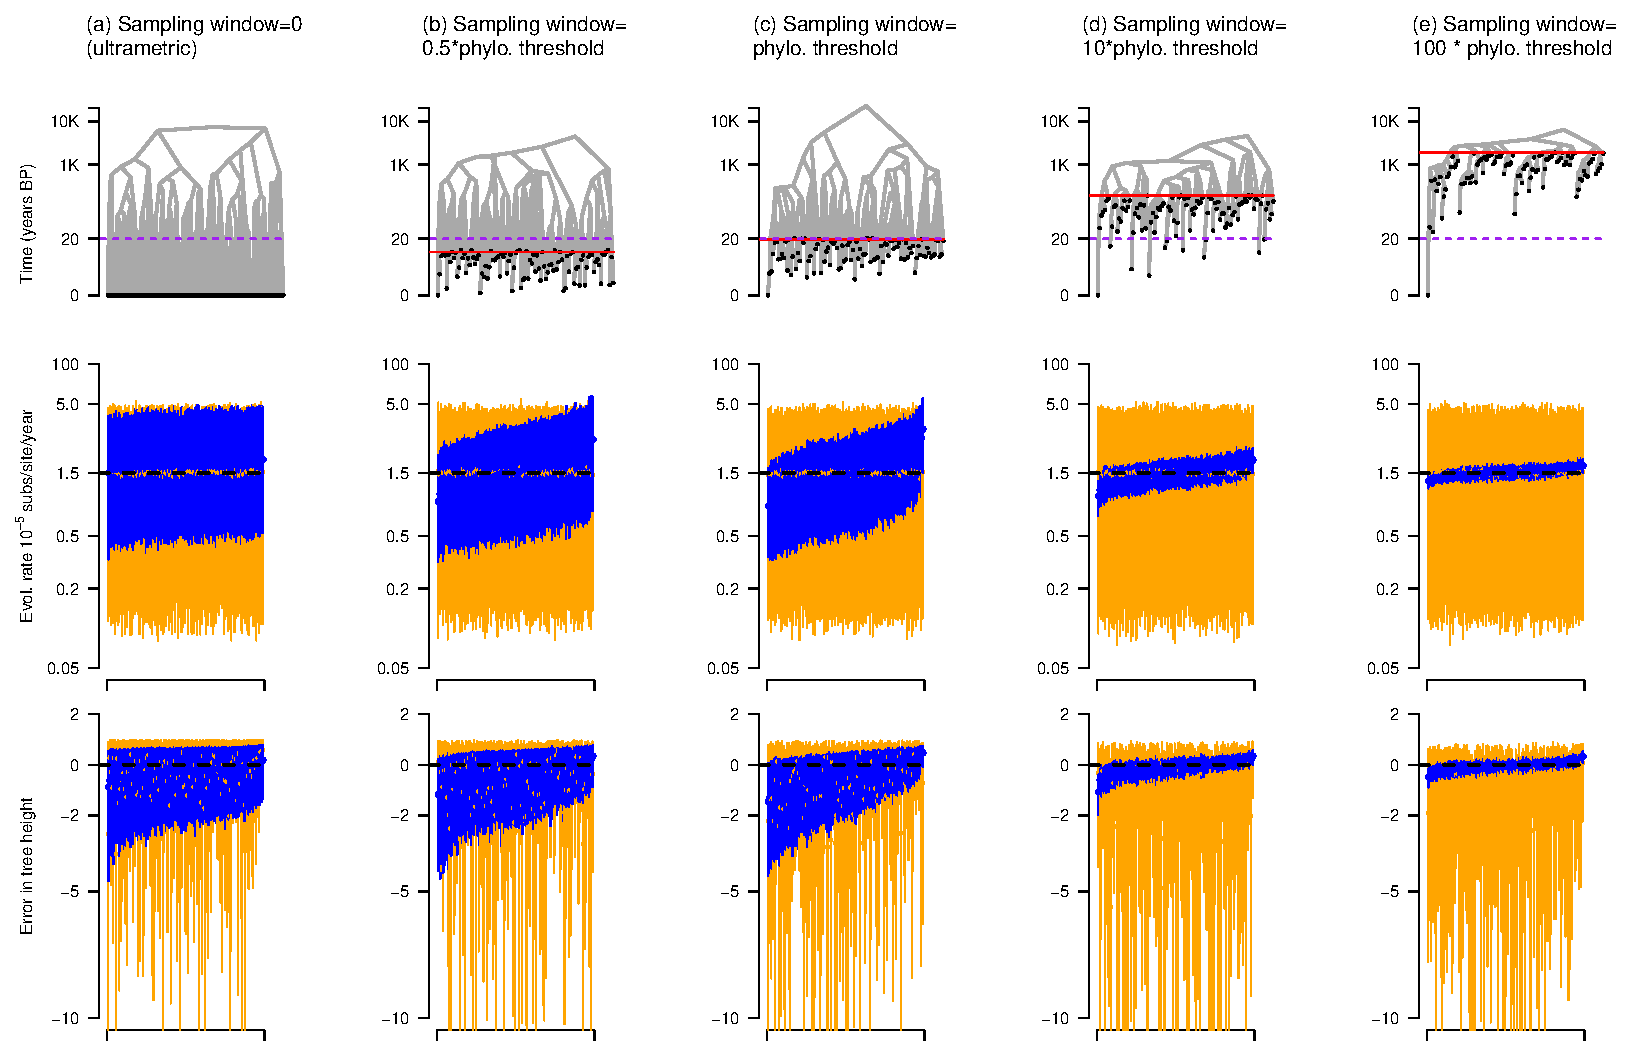
\includegraphics[scale=0.7, angle=0]{summary_all_estimates_correct_prior.pdf}
			\caption{Simulations of varying sampling window widths. Each column corresponds to a simulation setting: (a) is for ultrametric trees where all samples are collected at the same point in time, (b) is for the situation where the sampling window is 10 years (half the phylodynamic threshold), (c) is where the sampling window is exactly the phylodynamic threshold of 20 years. Scenarios (d) and (e) denote sampling windows that are 10 and 100 times the phylodynamic threshold. The first row is an example of a simulated phylogenetic tree with branch lengths scaled in units of time. The black circles represent genomic samples. The purple dashed line is is the phylodynamic threshold and the solid red line is for the oldest sample, such that it represents the sampling window. Note that time here is shown in log$_{10}$ scale. The second row is the estimated evolutionary rate over 100 simulations. The dashed black line is the value used to generate the data (i.e. the ground truth), the dark blue bars are the posterior, and those in orange are the prior. For the prior and the posterior we use solid circles to show the mean estimate and the width of the error bars denotes the 95\% quantile range. The third row is the estimate of the error in tree height (the age of the tree). The error in tree height is calculated as $\frac{true-estimated}{true}$.}
			\label{figure:Fig2}
		\end{center}
		%		\centering
	\end{figure}
\end{landscape}

\begin{landscape}
	\begin{figure}[H]
		\begin{center}
			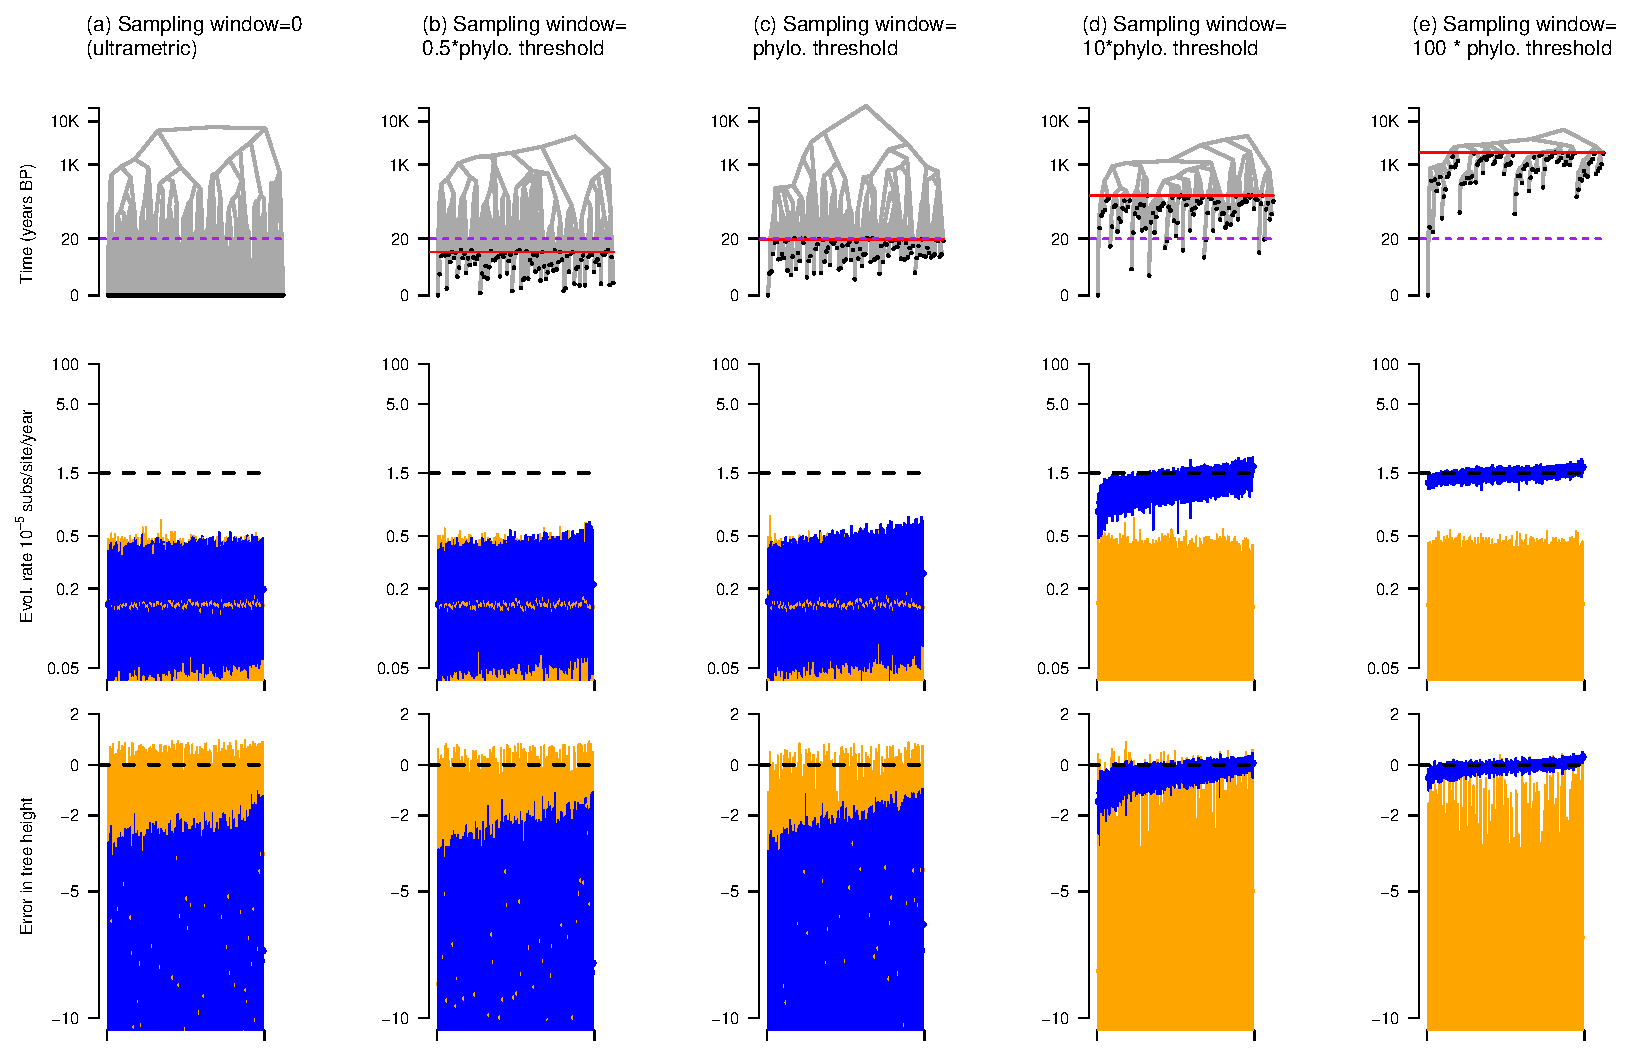
\includegraphics[scale=0.7, angle=0]{summary_all_estimates_misleading_prior.pdf}
			\caption{Simulations of varying sampling window widths. The colours, labels and legends match those from fig \ref{figure:Fig2}. However, in these analyses we deliberate use misleading priors on two key parameters, with a exponential distribution with mean 5,000 for the coalescent population size (true value=5,000), and a $\Gamma(shape=1.5, rate=10^{6})$ with mean=$1.5\times10^{-6}$ (true value=$1.5\times10^{-5}$).}
			\label{figure:Fig3}
		\end{center}
		%		\centering
	\end{figure}
\end{landscape}


\subsection{Temporal sampling bias}
We investigated the impact of temporal sampling bias on the precision and accuracy on molecular clock estimates. For this purpose we simulated data with the same genomic characteristics as HBV and where genome sampling was conducted over five periods of time uniformly distributed between the present and the root of the trees (fig. \ref{figure:Fig4}(a)). The fully sampled trees contained 500 genome samples, equally distributed over each of the five sampling times. Such stratified sampling is expected in ancient DNA studies, for example when a set of samples are drawn from archaeological sites (e.g. \cite{spyrou2019phylogeography}). We sampled the complete data sets by randomly selecting 20 samples from each strata, which we refer to as `time-uniform' sampling, and by sampling with a probability that is inversely proportional to the age of the strata, referred to as `time-biased'. The time-uniform and time-biased sampling strategies both contain 100 samples (1/5$^{th}$ of the complete data), but the time-biased only includes a small number of ancient samples.

The coverage of the evolutionary rate estimate was comparable across simulation treatments, at 88\% for the complete data set, 83\% for the time-uniform, and 89\% for the time-biased (fig. \ref{figure:Fig4}(b)). The somewhat higher coverage for the estimates from the time-biased analyses is likely because this sampling treatment reduces the precision of the posterior, rather than an improvement in both accuracy and precision.

We also calculated a measure of bias for both sampling strategies by counting the number of simulations for which the posterior mean with either sampling strategy was higher than that with the complete data. We found that 50\% of the estimates under time-uniform sampling had higher means than the complete data, while the same was true for 45\% of those with time-biased sampling (fig. \ref{figure:Fig5}(a)). Although these numbers do not indicate substantial bias, we do note that time-biased sampling tends to lead to lower mean evolutionary rate estimates than using the complete data or time-uniform sampling.

The most striking result of the temporal sampling strategies was in the precision of the posterior. Both sampling treatments resulted in posterior distributions that were wider than with the complete data, which is to be expected because they are effectively smaller data sets with less information. However, the time-biased sampling data sets almost invariably have posterior distributions that were less precise than those from the time-uniform sampling (Fig. \ref{figure:Fig5}(b)).

%\begin{landscape}
\begin{figure}[H]
	\begin{center}
		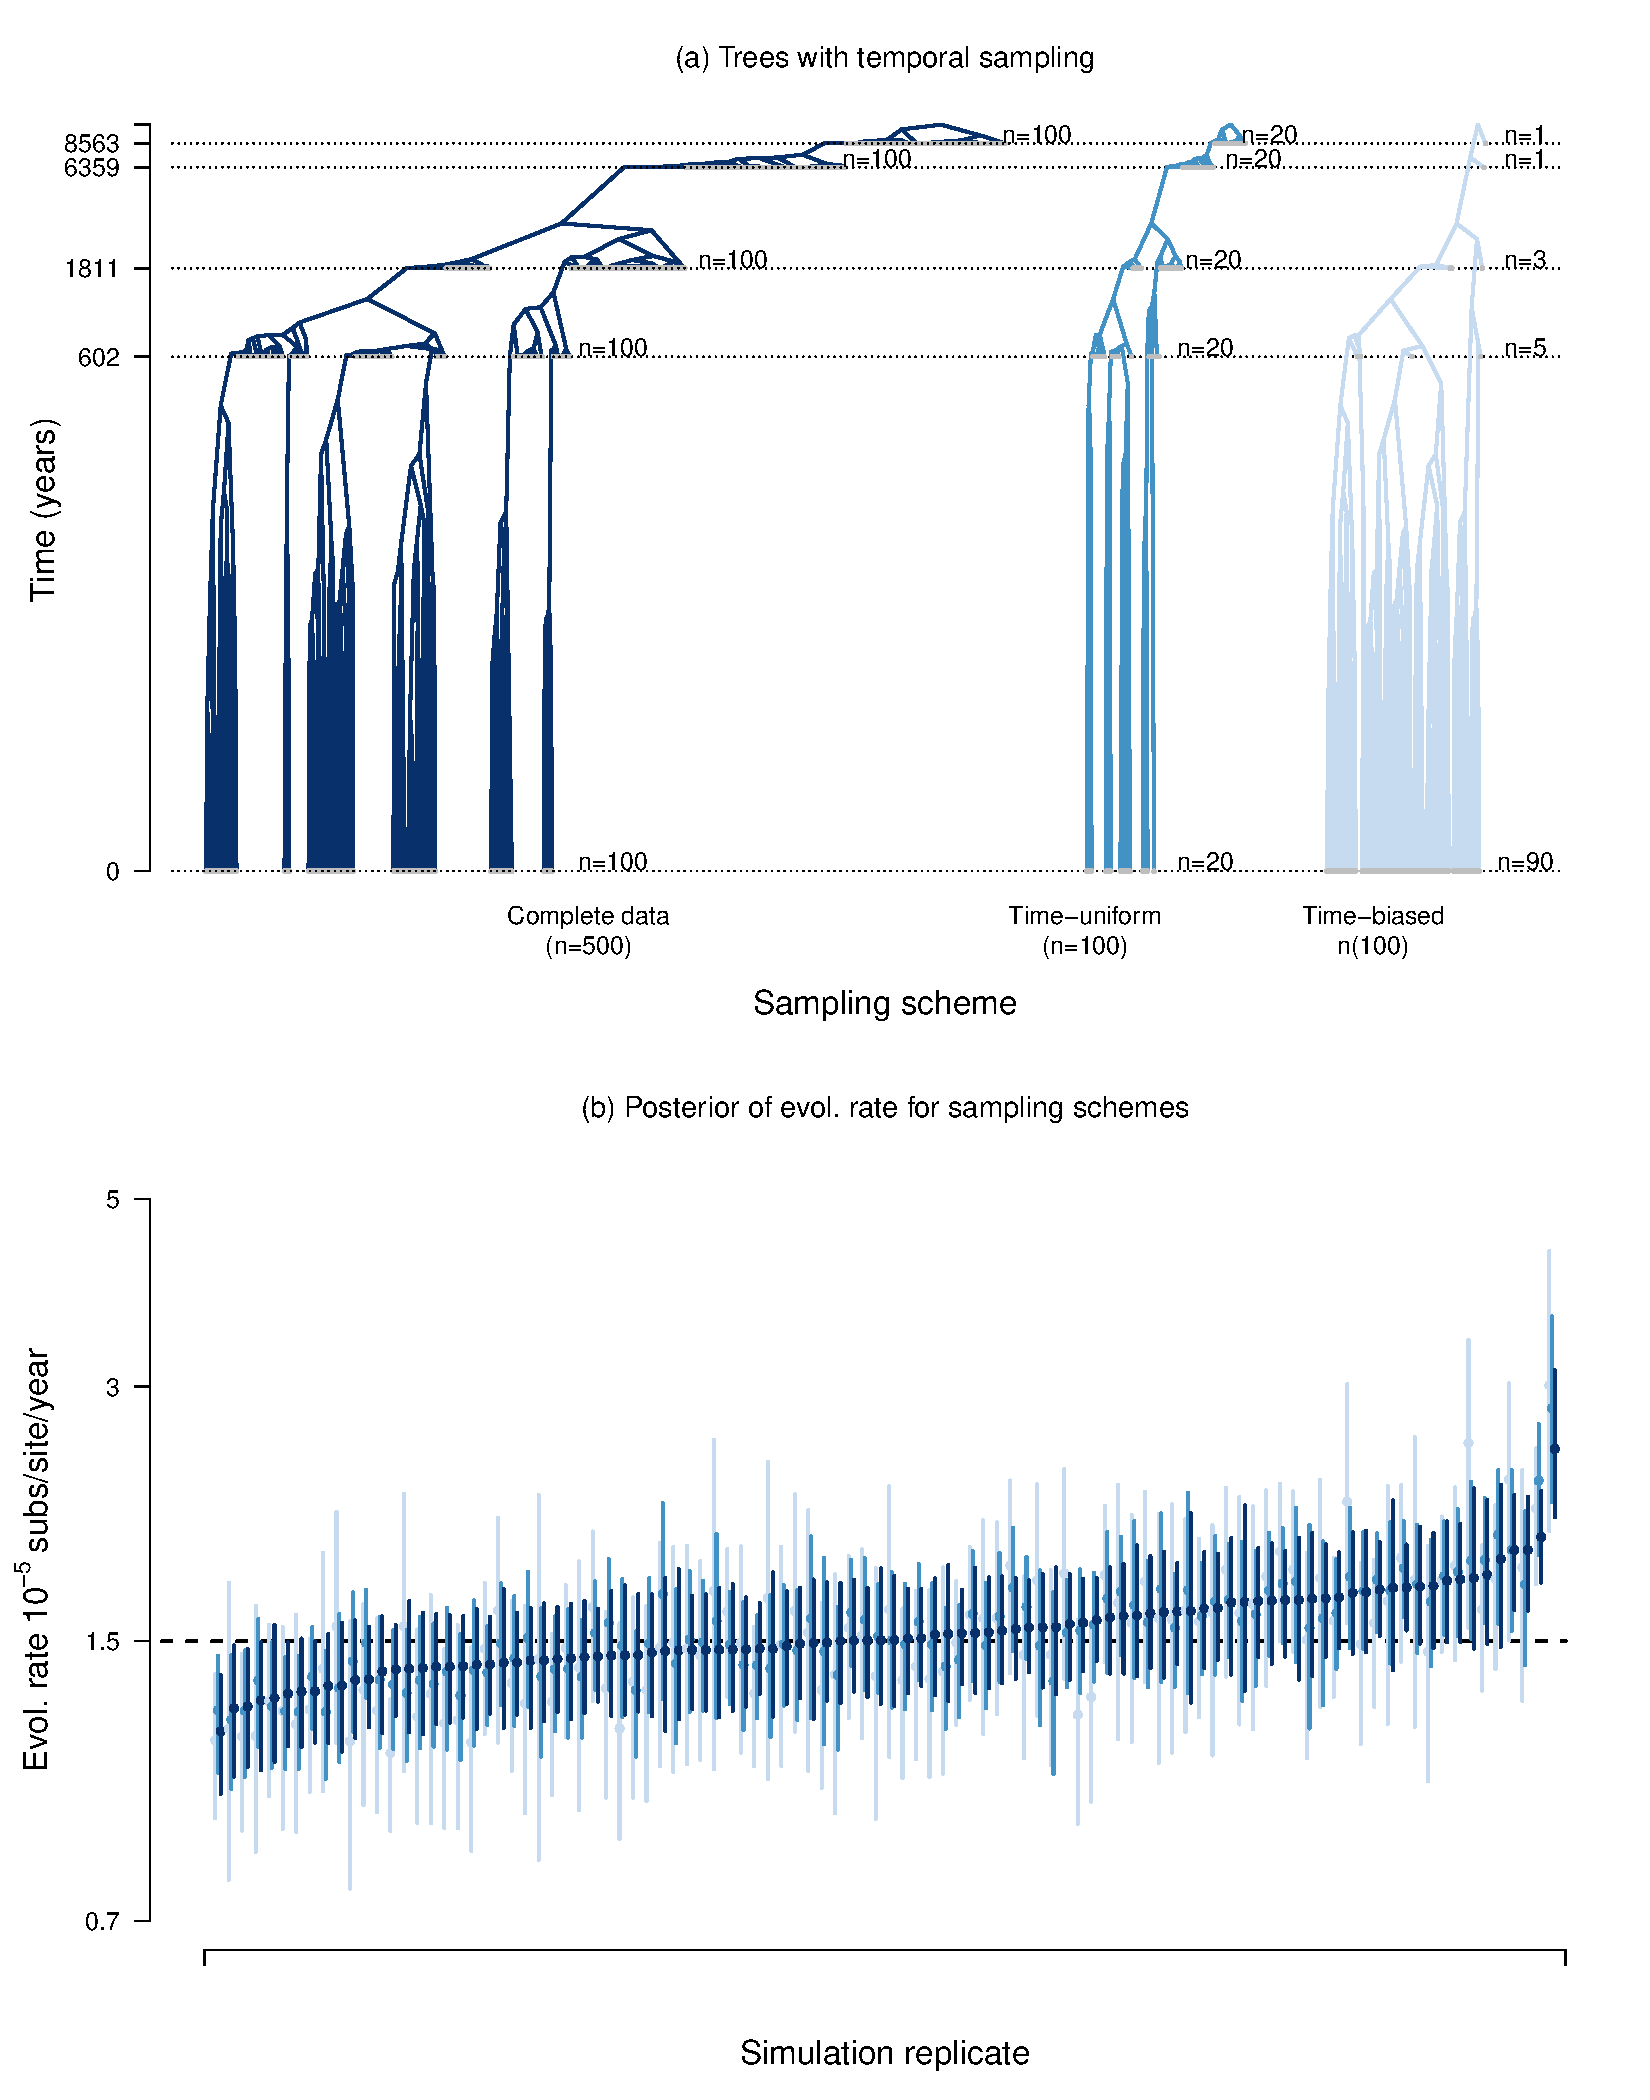
\includegraphics[scale=0.5, angle=0]{sampling_bias_summary_trees_rates.pdf}
		\caption{Analyses under sampling treatments over time. In (a) we show an example of a the trees for a simulation replicate, with branch lengths and time in log$_{10}$ scale. The complete data set consists of 500 genome samples, collected in five points in time, with an equal number of samples per time point (n=100). The first sampling strategy is unbiased, where 20 samples are drawn from each time point, and is known here as `time-uniform'. The `time-biased' regime is where sampling intensity decreases over time. Note that the total number of samples in the time-uniform and time-biased treatments is identical. In (b) we show the posterior estimates of the evolutionary rate for each treatment. Each simulation replicate is represented by three error bars: dark blue for the complete data, and lighter shades of blue for the estimates from the time-uniform and time-biased sampling treatments. The width of the error bars denotes the 95\% quantile range and the dots are the mean value. The dashed line shows the true value used to generate the data.}
		\label{figure:Fig4}
	\end{center}
		%		\centering
\end{figure}
%\end{landscape}


\begin{figure}[H]
	\begin{center}
		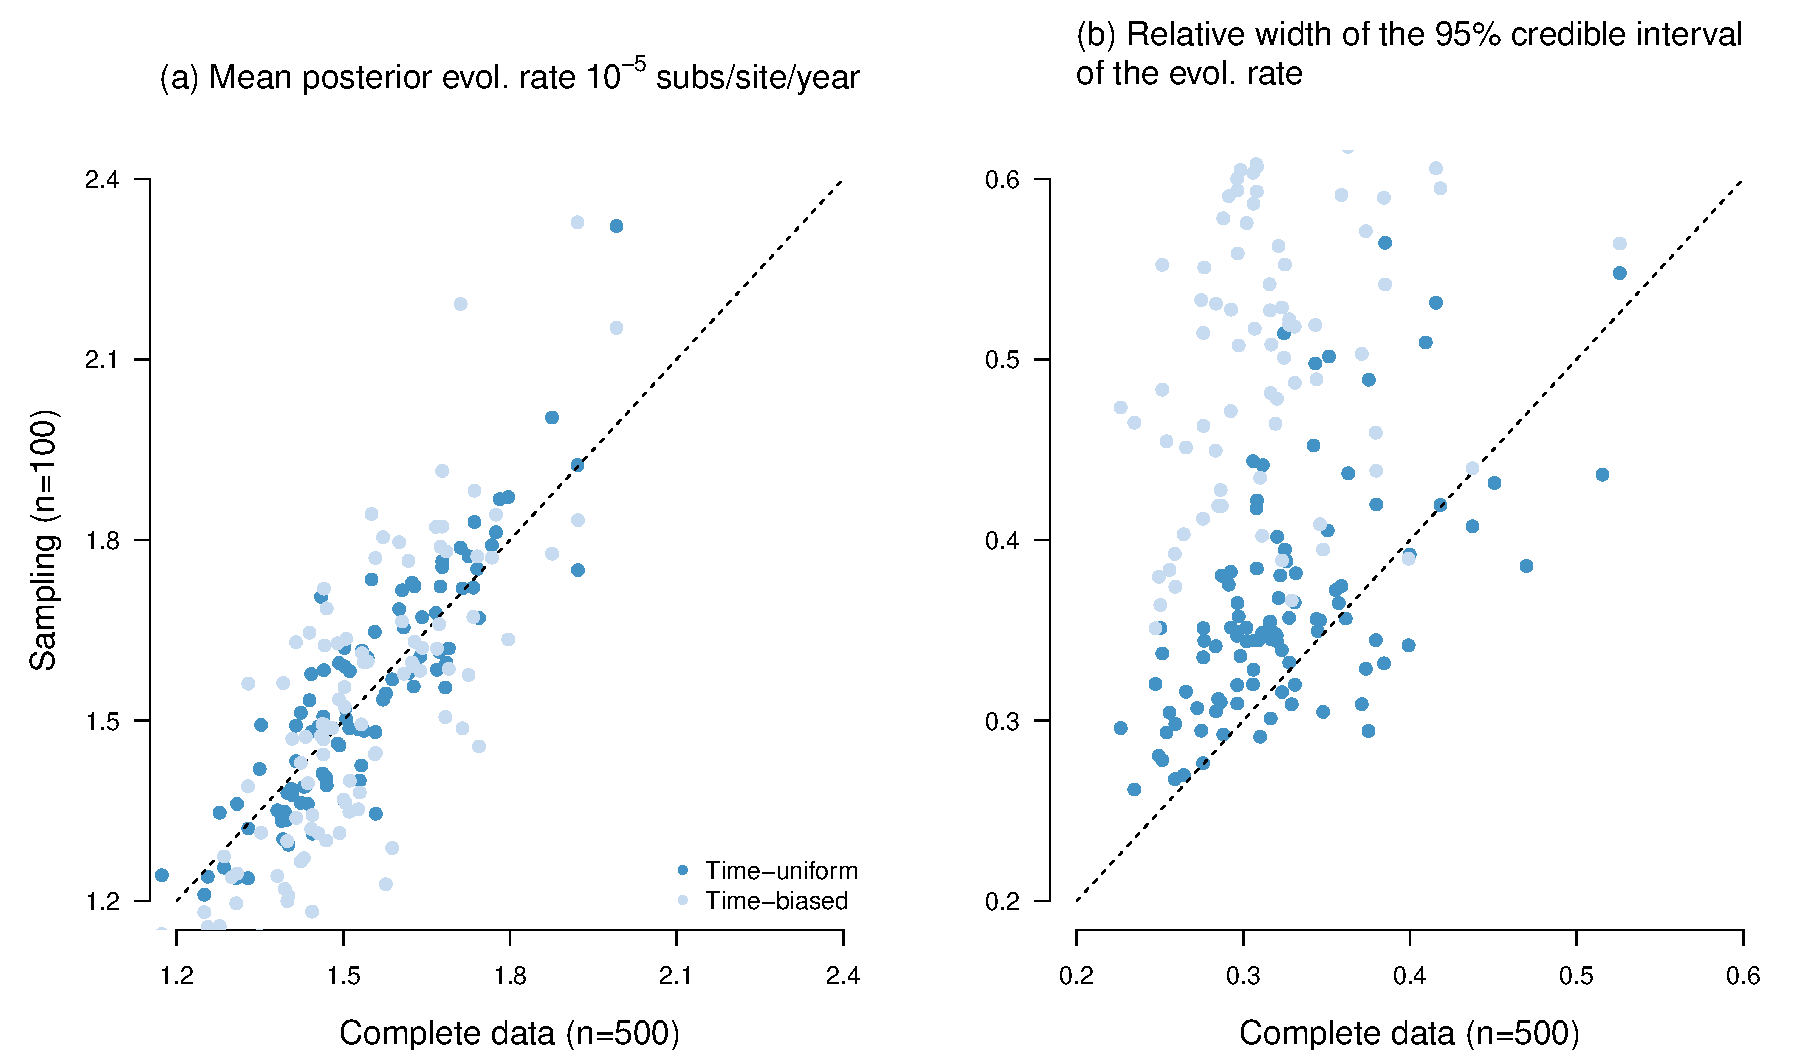
\includegraphics[scale=0.5, angle=0]{sampling_bias_summary_rates.pdf}
		\caption{Comparison of posterior estimates evolutionary rate estimates between complete data (x-axis) and two sampling treatments (y-axis), time-uniform (dark blue) and time-biased (light blue). Each dot is a simulation replicate. In (a) we show the mean posterior evolutionary rate estimate. Points that fall along the y=x line (dashed line) represent identical mean posterior for the sampling treatment and the complete data, while those above or below represent higher or lower estimates, respectively, relative to the complete data. In (b) we show the width of the credible interval (a measure of precision or uncertainty), calculated as the upper minus the lower 95\% credible interval range divided by the mean value. Values that fall along the y=x line denote those for which the complete data and either sampling strategies are equally precise, while those above and below the y=x line are more or less precise, respectively.}
		\label{figure:Fig5}
	\end{center}
	%		\centering
\end{figure}

\subsection{Empirical analyses of Hepatitis B virus (HBV) ancient and modern genomes}
To explore the impact of the width of the sampling window and the temporal sampling bias on the estimates of evolutionary rates and times, we performed analyses of a HBV data set that includes modern and ancient genomes, from \cite{kocher2021ten}. The complete data set consisted of 232 genomes of length 3,344 nucleotides and with a sampling window of 10,535 years. HBV is an ancient pathogen that has likely codiverged with human populations for thousands of years \citep{locarnini2021origins, zehender2014enigmatic, paraskevis2013dating, muhlemann2018ancient}, and thus its phylodynamic threshold has not been empirically established, as is the case for recent outbreaks, like SARS-CoV-2 \citep{duchene2020temporal}. 

For our first set of analyses we varied the width of the sampling window: we drew 100 genomes with different sampling window widths: 0 (only modern samples), up to 500, 1,000, or 5,000 years before present. Increasing the sampling window resulted in estimates of the evolutionary rate that were more precise and closer to the estimate from the complete data set (fig. \ref{figure:Fig6}). In contrast to our simulations, here we find that the evolutionary rate is estimated to be higher for shorter sampling windows. This pattern is consistent with the vagaries of evolutionary rate variation in this virus, particularly time-dependency \citep{vrancken2017accurate}. However, a more likely cause is the effect of the marginal prior -our analyses using the `misleading' prior configuration above indicate that broadening the sampling window reduces the sensitivity of the estimates to the prior (supplementary material online).

\begin{figure}[H]
    \begin{center}
        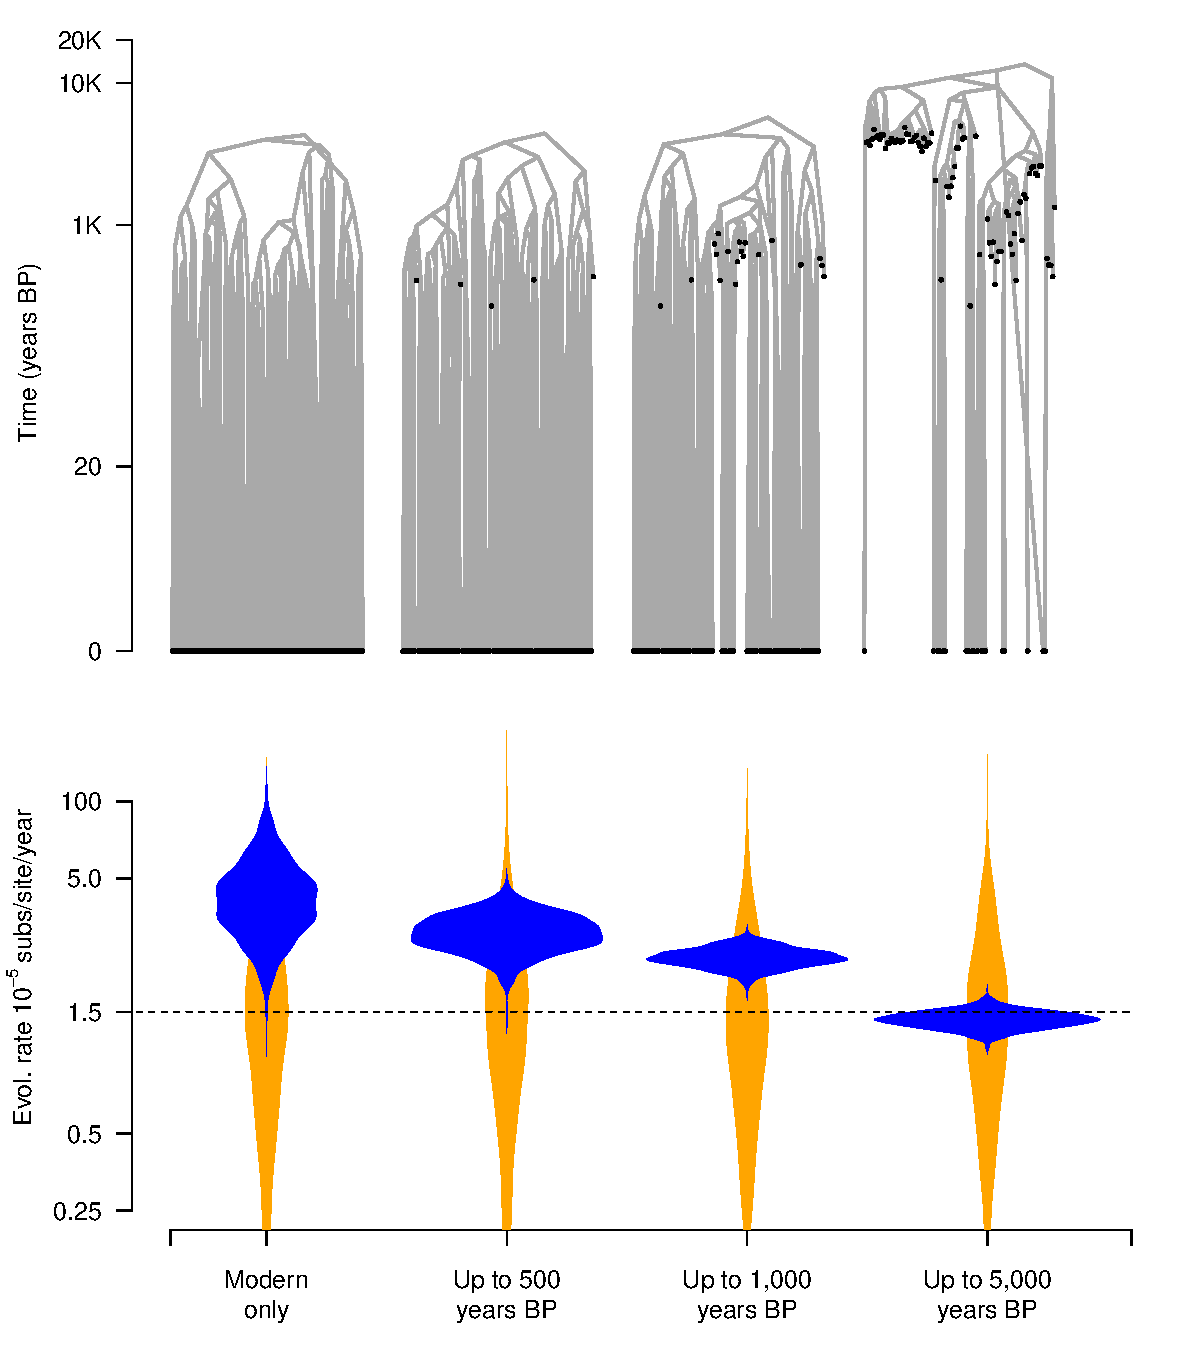
\includegraphics[scale=0.7, angle=0]{empirical_results_depth.pdf}
        \caption{Results from empirical analyses of Hepatitis B virus (HBV) ancient DNA data. The phylogenetic trees correspond to highest clade credibility trees from three analyses where the data were subsampled to increase the width of the sampling window progressively. First, we only consider modern samples, then those up to 500, 1,000, and 5,000 years before present. In all cases the data sets consist of 100 genome samples. The violin plots show the posterior distribution of the evolutionary rate in blue and its corresponding prior in orange. The dashed line shows the mean evolutionary rate estimate from the complete data set.}
        \label{figure:Fig6}
    \end{center}
    %		\centering
\end{figure}

For our second set of empirical analyses, we subsampled the data to produce a range of temporally biased sampling scenarios. We varied the proportion of modern samples, from 95\% to 10\%, while retaining the original sampling window width of the original study of 10,535 years. Each data set consisted of 100 genomes, such that they only differ in the distribution of modern and ancient samples (fig. \ref{figure:Fig7}). 

The impact of temporal sampling bias was less clear than in our simulations above (figs \ref{figure:Fig4} and \ref{figure:Fig5}). The data set with 95\% modern genomes had the highest uncertainty in the evolutionary rate estimate, but uncertainty did not decrease monotonically with the proportion of modern genomes. Moreover, the posterior estimate of the evolutionary rate from the data set with 50\% modern genomes deviated the most from the that obtained using the full data set. Critically, when we analysed these data using the `misleading' prior setting we found that increasing the number of ancient samples resulted in a less influential prior. These results demonstrate that the exact impact of temporal sampling bias may be difficult to predict in practice, but that generally increasing the number of ancient samples results in data sets that are more informative, in that the difference between the prior and posterior is more pronounced than when only a few ancient samples are available.

\section{Discussion}
\textcolor{red}{DRAFT UP TO HERE}
\begin{itemize}
    \item On the phylodynamic threshold. That it is a useful concept. However it is not a discrete bound, but a region. When the prior is `correct', sampling over longer time periods (past the threshold) simply improves precision. When the prior is misleading, we may well need to sample beyond the threshold. In our case, we found that sampling 10 times more was required to overcome the misleading prior. If the prior is reasonable, then sampling less than the phylodynamic threshold is OK.
    \item Tests of temporal signal are important, but they only quantify the strength of the association between dates and genetic distance. However, prior sensitivity analyses appear to be even more important. For example, we could sample at the phylodynamic threshold, in which case most tests would likely suggest temporal signal. However, if the prior is misleading (even if we consdier it uninformative) then it might still obscure the signal from the data. A reasonable approach would be to consistently check the prior on a few key parameters, notably the evolutionary rate and the height of the tree. Ideally, the posterior should be more precise than the prior.
    \item Sampling bias is an obvious concern. Here we do not focus on population structure, which has been investigated previously and causes X. Instead we focus on temporal sampling bias, which is a common concern in aDNA data sets. Contrary to our expectations, it does not seem to lead to a systematic bias, given the the prior is not misleading, but instead it simply improves information content in the data. This is good, but determining whether the data are sufficiently informative is tricky, and thus choosing a good prior is important. 
    \item a short discussion on the clock rate prior and tree prior (ctmc rate reference, the gamma here, the colescent, the birth-death).
    
\end{itemize}



\begin{figure}[H]
    \begin{center}
        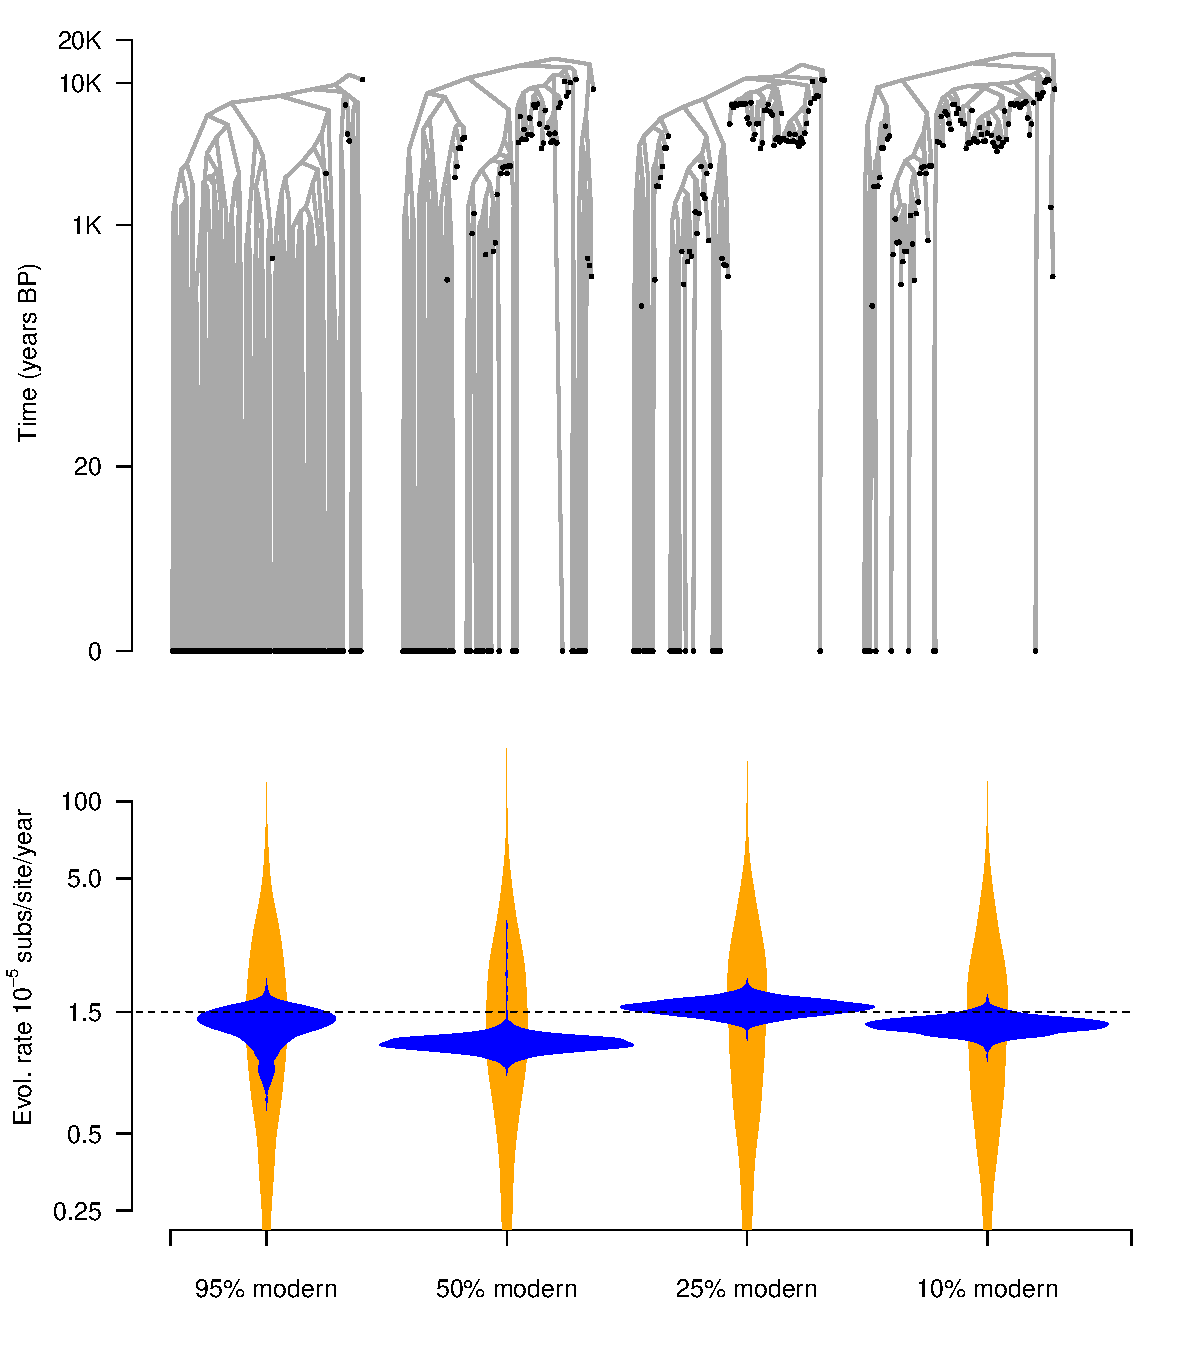
\includegraphics[scale=0.7, angle=0]{empirical_results_biased.pdf}
        \caption{Results from empirical analyses of Hepatitis B virus (HBV) ancient DNA data. The phylogenetic trees correspond to highest clade credibility trees from three analyses where the data were subsampled to include an increasing number of ancient samples. First, we consider a data set for which the samples are are 95\% modern and the remaining 5\% being the most ancient. Then, we reduce the number of modern samples to 50\%, 25\% and 10\%, and the rest being ancient. Note that the sampling window is constant because we always retain the most ancient samples. In all cases the data sets consist of 100 genome samples. The violin plots show the posterior distribution of the evolutionary rate in blue and its corresponding prior in orange. The dashed line shows the mean evolutionary rate estimate from the complete data set.}
        \label{figure:Fig7}
    \end{center}
    %		\centering
\end{figure}



\section{Materials and methods}
\subsection{Simulations}
\subsubsection{Data generation}
We simulated phylogenetic trees and the evolution of nucleotide sequences to assess the impact of varying the sampling window and temporal sampling bias. We parameterised our simulations to resemble an HBV population evolving over 10,000 years before present, as described by \cite{kocher2021ten}. 

We generated phylogenetic trees under a coalescent process in which the population size has been constant over time using the package ReMaster \citep{vaughan2024remaster}, part of the BEAST 2 (version 2.7) software. We set the population size to 5,000, which results in trees with an average age of 10,000 time units (years). The number of samples (i.e. tips) drawn from the trees and their ages was defined in ReMaster, according to the particular simulation scenario described below.

The simulation of sequence data requires trees with branch lengths in units of subs/site, instead of time. For this purpose, we multiplied the branch lengths of the trees by a lognormally distributed random variable with parameters $\mu=log(1.5\times10^{-5}) - \frac{0.25^2}{2}$ and $\sigma=0.25$. This procedure equates to simulating an uncorrelated relaxed molecular clock model with an underlying lognormal distribution \citep{drummond2006relaxed} with mean of $1.5\times10^{-5}$ subs/site/year and a standard deviation of 0.25. Because we multiply the branch lengths in units of years by a variable in subs/site/year, the resulting trees have branch lengths in units of subs/site, formally known as phylograms, in contrast to chronograms where the branch lengths correspond to time.   We obtained sequence alignments using the R package phangorn (v2.8.1) \citep{schliep2011phangorn}, according to a HKY+$\Gamma_4$ substitution model, with parameters $\kappa=2$, $\alpha=4$, and equal base frequencies. The alignmetns consisted of 3,200 nucleotides to match the average genome size of HBV.

We considered the phylodynamic threshold of our data to be about 20 years. For our simulations where we varied the sampling window, we set the ages of 100 tips to be sampled at present (all have an age of 0), or to be drawn from a uniform distribution between 0 and 10 (1/2 of the phylodynamic threshold), 0 and 20, 0 and 200, or 0 and 2,000. 

To investigate the impact of temporal sampling bias we initially simulated trees with 500 tips with sampling times distributed in 5 time points, with 100 tips per time point. The distribution of sampling times followed an exponential distribution with mean of 4,000, such that sampling times were concentrated towards the present. We simulated these complete trees in ReMaster. We followed the procedure above to simulate a molecular clock model and sequence alignments. 

We conducted two sampling schemes for the trees with 500 tips: the `time-uniform' scheme consisted of drawing 20 samples from each time point, whereas the `time-biased' scheme included of mostly modern samples (90 from the present, and 5, 3, 1, and 1 from the remaining time points). For each simulation scenario we generated 100 replicates.

\subsubsection{Simulated data analysis}

\textcolor{red}{MENTION SUBSAMPLING OF THE COMPLETE TREES AND THAT EACH SIMULATION SETTING HAD 100 REPLICATES.}

Pending.

\section{Author contributions}
Pending.

\section{Competing interests}
Pending.


\section{Acknowledgments}
Pending.



%\bibliographystyle{plain}
\bibliography{References}

\end{document}